\documentclass[conference]{IEEEtran}
\IEEEoverridecommandlockouts

\usepackage{cite}
\usepackage{amsmath,amssymb,amsfonts}
\usepackage{graphicx}
\usepackage{textcomp}
\usepackage{xcolor}
\usepackage{booktabs}
\usepackage{multirow}
\usepackage{array}
\usepackage{url}
\usepackage{placeins}
\usepackage[utf8]{inputenc}
\usepackage{newunicodechar}
\newunicodechar{，}{,}


\def\BibTeX{{\rm B\kern-.05em{\sc i\kern-.025em b}\kern-.08em
    T\kern-.1667em\lower.7ex\hbox{E}\kern-.125emX}}

\begin{document}

\title{Group 11: Detection of Body-Focused Repetitive Behaviors Using Deep Learning and NLP-Based Models}

\author{
\IEEEauthorblockN{
Gan Song,
Jia Min,
Yuan Guo,
Jinqiang Ding,
Zixuan Xu
}
\IEEEauthorblockA{
Fairleigh Dickinson University, Vancouver, BC, Canada \\
\{g.song@student.fdu.edu, j.min@student.fdu.edu, y.guo4@student.fdu.edu, j.ding2@student.fdu.edu, z.xu9@student.fdu.edu\}
}
}

\maketitle

\begin{abstract}

Body-focused repetitive behaviors (BFRBs) such as hair pulling, skin picking, and scratching can cause physical harm and psychosocial difficulties. Automatic detection of these behaviors using wearable sensor data can support earlier intervention and biofeedback-based management. Existing work has shown that multimodal sensing with IMU, thermopile, and time-of-flight (TOF) signals is promising for distinguishing BFRBs from non-BFRB gestures, but performance remains uneven across model types and fine-grained gesture classes.

In this work, we reproduce the main deep learning baselines from the prior study and extend them with NLP-inspired sequence models for BFRB detection. We compare classical frequency-domain models, CNN-BiLSTM architectures, fusion strategies, and transformer-style sequence models under a unified evaluation pipeline. Our best reproduced baseline achieves a binary F1-score of 95.68\%, while our best NLP-based model achieves a macro-averaged F1-score of 60.70\%, demonstrating that NLP-inspired sequence models can improve fine-grained classification performance while maintaining strong binary detection accuracy.
\end{abstract}

\clearpage

\section{Introduction}

Body-focused repetitive behaviors (BFRBs), such as hair pulling, skin picking, and nail biting, are chronic self-directed habits that can lead to significant physical injury and deep psychosocial distress \cite{woods2022prevalence}. These behaviors are prevalent among individuals with anxiety disorders and obsessive-compulsive disorder (OCD), and they often serve as key indicators of underlying mental health challenges \cite{stein2019ocd}. Recent clinical surveys highlight that nearly 97.1\% of individuals have engaged in at least one compulsive repetitive behavior during their lifetime, with 24\% reporting that these actions caused them actual physical harm or clinically meaningful impairment \cite{stein2019ocd}. Despite their high prevalence, BFRBs often go untreated because they frequently occur during periods of semi-awareness, which makes self-monitoring extremely difficult for patients. In many cases, individuals are not fully conscious of when the behavior starts, how frequently it occurs, or what triggers it in everyday life. This makes early intervention difficult and limits the effectiveness of treatments that rely heavily on self-reporting or retrospective behavioral recall. Consequently, there is an urgent need for automated detection systems that can provide real-time biofeedback, enabling individuals to manage their habits through immediate intervention and digital monitoring \cite{lee2023bfrb}.


Existing state-of-the-art approaches mainly rely on frequency-domain processing of sensor streams, such as Fast Fourier Transform (FFT) features, combined with classifiers including multilayer perceptrons (MLPs) and random forests, as well as specialized TOF-based sequence models and multimodal fusion architectures \cite{zhang2025baseline}. While these approaches achieve strong performance on binary detection, with the best late-fusion baseline reaching a binary F1-score of 96.86\%, their performance drops considerably in fine-grained classification settings \cite{zhang2025baseline}. Specifically, macro-averaged F1-scores for multi-class gesture recognition remain below 60\%, highlighting the difficulty of distinguishing among behavior classes with similar motion trajectories and contact patterns \cite{zhang2025baseline}. This gap suggests that current methods are better at learning coarse decision boundaries than at capturing the subtle temporal structure needed for detailed gesture discrimination. In practice, distinguishing whether a gesture is harmful is easier than identifying its exact type, since several BFRB classes involve similar arm movement patterns and differ only in fine contact location, temporal duration, or subtle approach-and-withdrawal behavior.

One possible reason for this limitation is that frequency-domain summaries, while effective for capturing global signal regularities, may partially obscure the temporal ordering of events within a gesture sequence. For wearable sensor data, however, the progression of a gesture often carries important information. The approach toward the face or neck, the short moment of contact, and the repeated local motion that follows may all be crucial for differentiating one BFRB from another. In particular, frequency-domain summaries may not fully preserve the temporal evolution and non-stationary dynamics of wearable sensor sequences, and simpler recurrent models may lack sufficient capacity to model long-range dependencies across complex gestures. These limitations motivate the exploration of more expressive sequence modeling approaches inspired by natural language processing.

To alleviate these issues, we propose a design that extends beyond traditional frequency-domain analysis by adopting sequence modeling techniques inspired by modern Natural Language Processing (NLP) \cite{vaswani2017attention}. Our approach treats multimodal sensor data as tokenized sequences, allowing the model to capture both short-range sensor motifs and global temporal dependencies. Instead of compressing the full gesture too early into a static summary, these models preserve the ordered structure of sensor readings and learn how local temporal fragments interact across the entire sequence. This viewpoint is particularly useful for BFRB recognition because the meaning of a gesture depends not only on which sensor values are observed, but also on when they occur and how they evolve over time.

We implement and evaluate several advanced architectures, including Gated Recurrent Units (GRU), attention-enhanced Long Short-Term Memory (LSTM) networks, and Temporal Convolutional Networks (TCN) \cite{hochreiter1997lstm, cho2014gru, lea2017tcn}. Central to our design is the use of a self-attention mechanism, which allows the network to dynamically weight the most informative time steps within a gesture sequence, such as the specific moment of skin contact \cite{vaswani2017attention}. This mechanism helps the model focus on discriminative temporal segments rather than treating all parts of the sequence as equally important. By integrating spatial feature extraction with sequential modeling in a hybrid framework, our solution aims to enhance the discriminative power for fine-grained gesture classification, thereby providing more reliable and detailed feedback for BFRB management.

The main contributions of this work are as follows:
\begin{itemize}
    \item We successfully reproduce key experimental baselines for BFRB detection, confirming that the late fusion baseline achieves a binary F1-score of 96.86\% and a macro F1-score of 58.89\% \cite{zhang2025baseline}.
    \item We design and implement multiple NLP-inspired sequence models, including GRU, attention-enhanced LSTM, and TCN architectures, to model the complex temporal dynamics of multimodal sensor data.
    \item We evaluate a Transformer-based sequence model that utilizes self-attention to interactively capture global dependencies across sensor streams \cite{vaswani2017attention}.
    \item We demonstrate that our proposed LSTM-Attention model achieves a binary F1-score of 97.26\%, slightly outperforming the existing state-of-the-art fusion-based models.
    \item We show that our hybrid CNN-Token-LSTM model achieves an improved macro-averaged F1-score of 60.71\%, validating the effectiveness of token-based sequential modeling for fine-grained gesture recognition.
\end{itemize}

\clearpage
\section{Background}

\subsection{TOF Sequence Representation}

In the Helios dataset, each gesture is represented as a temporal sequence of sensor readings rather than as a single independent frame. This sequence formulation is important because gesture recognition depends on how sensor measurements evolve over time. The Helios device includes five TOF sensors, and the released dataset flattens their readings into 320 TOF features per time step \cite{zhang2025bfrb}.

TOF data can therefore be modeled as a multivariate time series, where measurements belonging to the same gesture are grouped into an ordered sequence. Since gesture sequences have variable lengths, they are padded or truncated to a fixed size for batch processing. A binary mask is used to distinguish valid time steps from padded positions, ensuring that padding does not affect model computation. This representation preserves temporal structure while providing a consistent input format for sequence models. Figure~\ref{fig:tof_wavelet_transformer} shows how TOF readings are organized into fixed-length sequences, transformed by a wavelet operation, and encoded by a Transformer with masking and positional encoding.

\begin{figure}[!htbp]
    \centering
    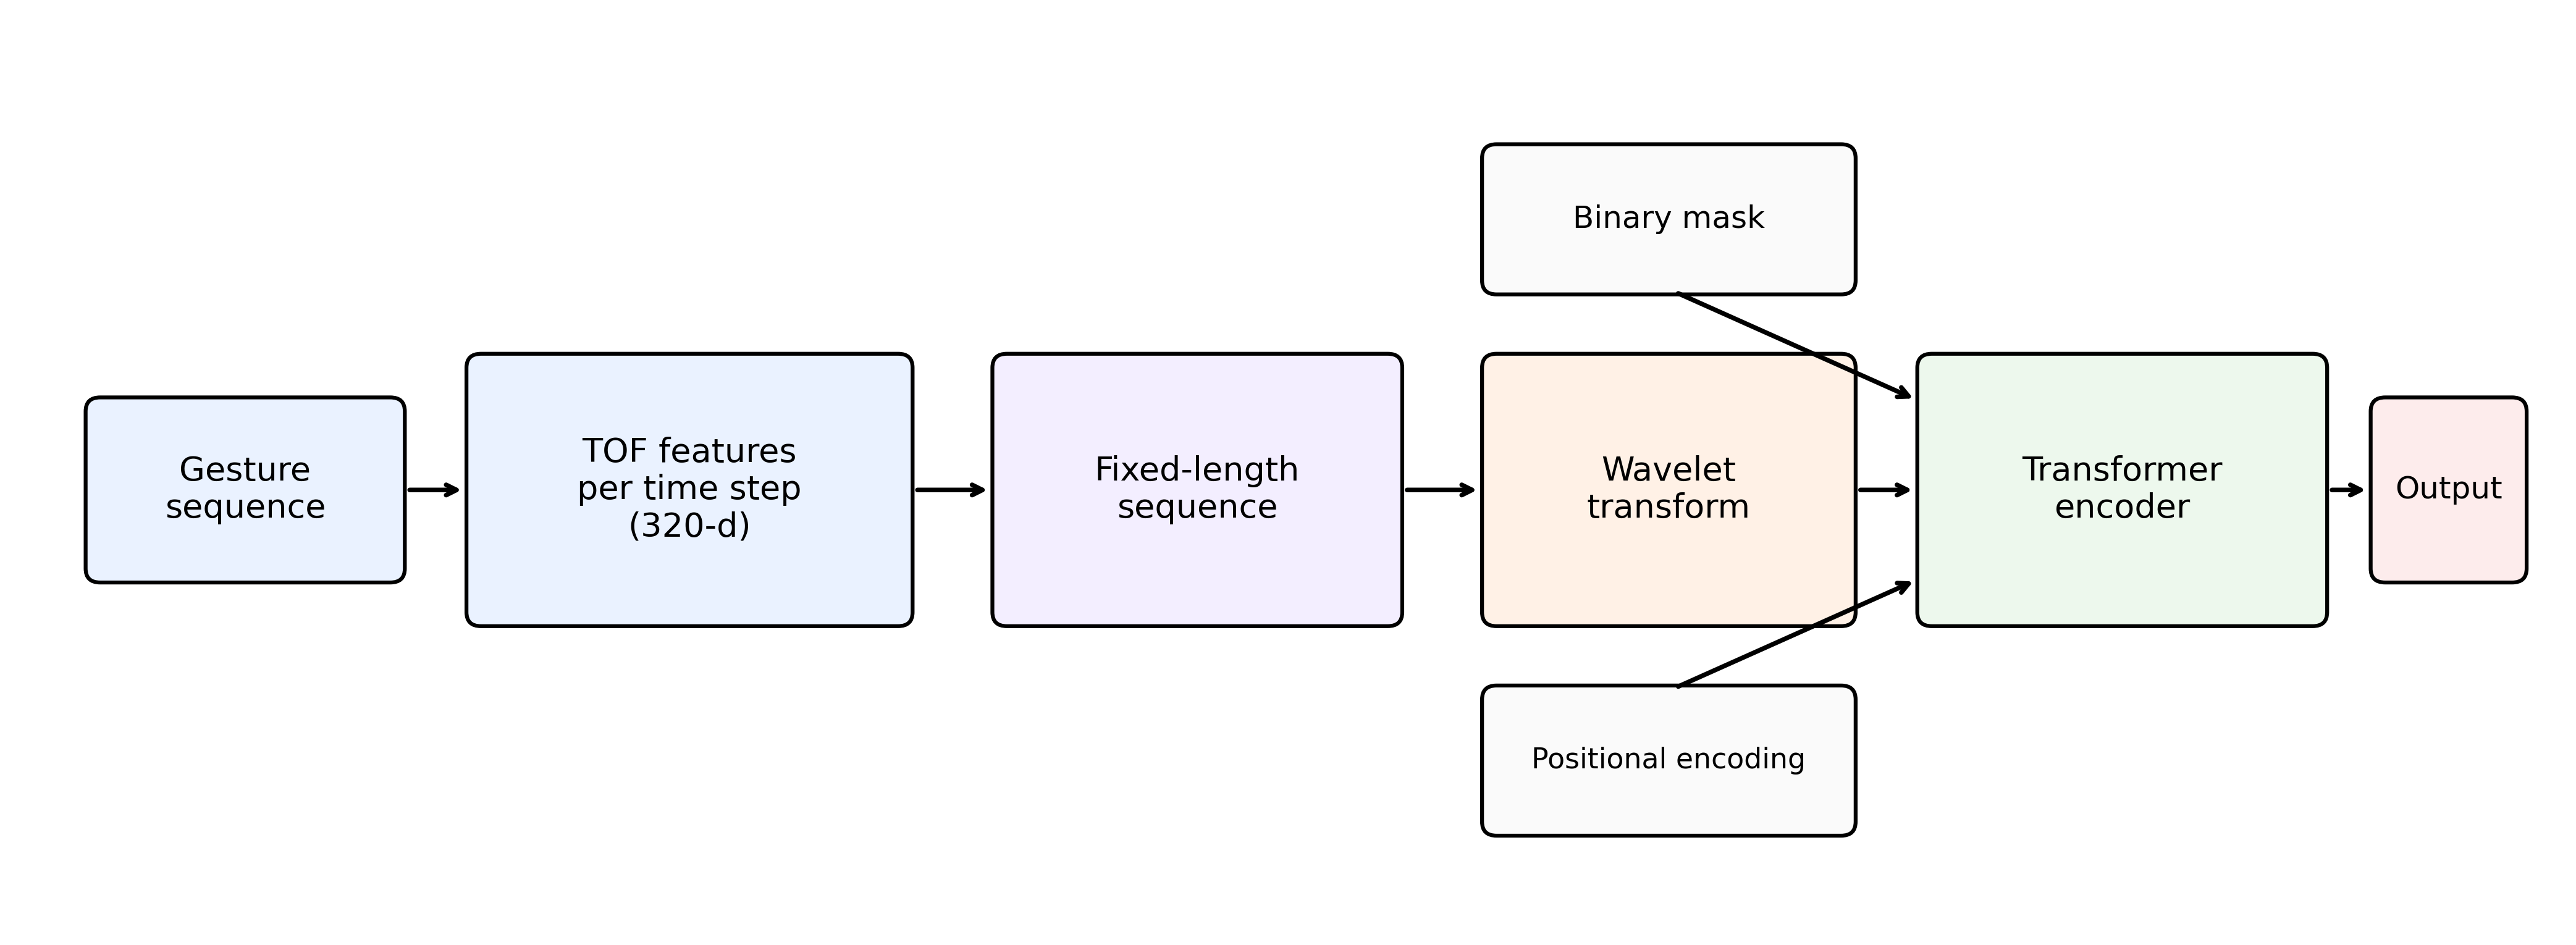
\includegraphics[width=\columnwidth]{tof_wavelet_transformer (2).png}
    \caption{Illustration of TOF sequence representation, wavelet transform, and Transformer-based sequence modeling.}
    \label{fig:tof_wavelet_transformer}
\end{figure}

\subsection{Transformer Encoders for TOF Sequence Modeling}

To model TOF sequences, a Transformer encoder is adopted. Transformer models rely on self-attention, which allows each time step to directly interact with all others in the sequence \cite{vaswani2017attention}. This is particularly useful for gesture recognition, where the class label depends on temporal relationships across the full motion rather than on a single frame.

Since self-attention does not inherently preserve temporal order, positional encoding is introduced to provide sequence information. In addition, when sequences are padded to a common length, masking is required so that padded positions do not influence attention computation or the final sequence representation. These components together provide an effective framework for modeling variable-length TOF gesture sequences.

\subsection{Temporal Convolutional Networks for Sequence Modeling}

Temporal Convolutional Networks (TCN) provide another approach to modeling sequential data by using stacked one-dimensional convolutional layers. Unlike recurrent architectures, TCNs operate through convolutional filters applied along the temporal dimension, enabling parallel computation and efficient training \cite{bai2018empirical}. A key component of TCNs is the use of dilated convolutions. It expands the receptive field without increasing the number of parameters significantly, which allows the model to capture long-range temporal dependencies while maintaining computational efficiency. 

This is very useful for gesture recognition tasks, where both local motion patterns and longer temporal structures contribute to accurate classification. By capturing fine-grained temporal variations as well as global sequence dynamics, TCNs are well suited for multivariate sensor data such as IMU and thermopile signals. Besides that, since gesture sequences are padded or truncated to a fixed length for batch processing, TCN can process these sequences efficiently in parallel. This makes them a practical and scalable choice within our pipeline, especially when handling large-scale time-series data.

\subsection{LSTM Sequence Modeling Based on Attention Mechanism}

Recurrent neural networks, especially Long Short-Term Memory (LSTM) models, are widely used for sequence modeling because of their ability to capture long-term temporal dependencies \cite{hochreiter1997lstm}.

However, standard LSTM models compress the entire sequence into a single hidden layer representation, which limits their ability to focus on the most informative time steps. To address this limitation, attention mechanisms are introduced, assigning different weights to different parts of the sequence \cite{bahdanau2015attention}.

As shown in Figure ~\ref{fig:lstm_attention}, the input sequence is first processed by an LSTM to generate hidden states. Then, an attention layer weights these hidden states and aggregates them into a context vector that emphasizes important temporal information.

This is particularly important in gesture recognition tasks, as only certain segments of the sequence have high discriminative power. By combining LSTM with an attention mechanism, this model is able to better focus on key temporal regions while preserving sequence structure.

Compared to Transformer-based models \cite{vaswani2017attention}, LSTMs with attention mechanisms are more lightweight and introduce stronger sequence inductive bias, which is more advantageous for small datasets.

\begin{figure}[!htbp]
    \centering
    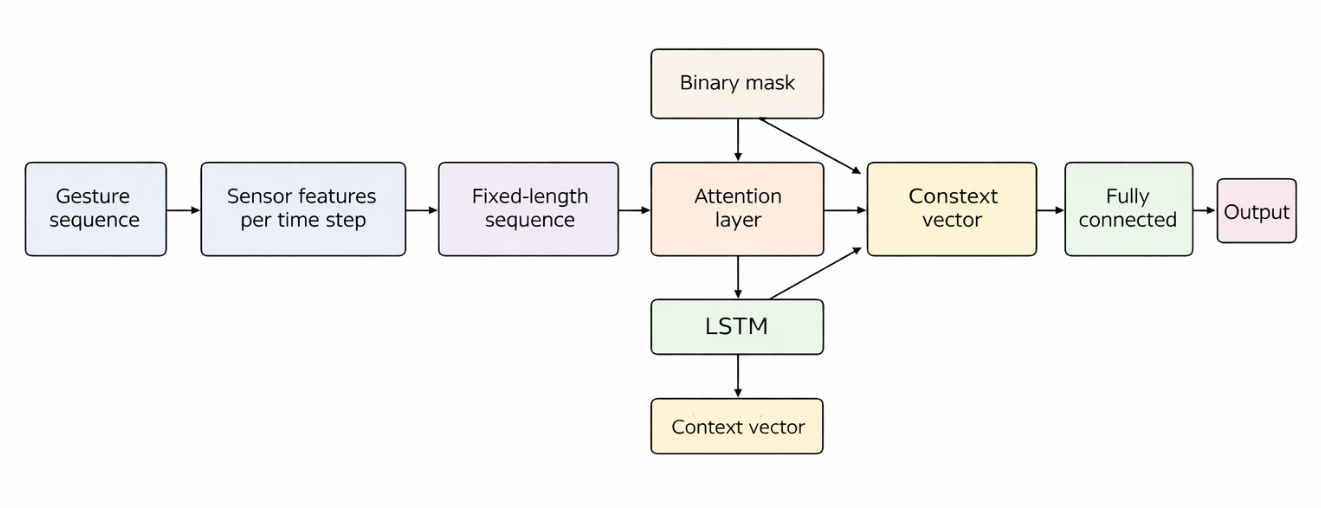
\includegraphics[width=\columnwidth]{Illustration of LSTM with attention mechanism for sequence modeling.png}
    \caption{Illustration of LSTM with attention mechanism for sequence modeling.}
    \label{fig:lstm_attention}
\end{figure}

\subsection{Token-LSTM modeling for TOF inputs only}

Inspired by natural language processing, our work treats each TOF sequence as a structured sequence of token-like representations. In Token-LSTM modeling for TOF inputs only, each time step is discretized into a symbolic token and mapped into an embedding space. Concretely, at each time step, the TOF sensor produces a high-dimensional vector such as 320 values. Instead of directly feeding this raw vector into a neural network, we summarize its statistical characteristics such as mean, standard deviation, minimum, and maximum, and then discretize these values into bins. Each combination of these discretized features is assigned a unique integer identifier that serves as a token. After this step of discretization, the sequence of tokens is passed through an embedding layer. The embedding layer maps each token index to a dense vector in a continuous space such as a 64-dimensional vector. These embedding vectors capture similarities between tokens: tokens corresponding to similar sensor patterns will have similar vector representations. After that, an LSTM captures temporal dependencies across the sequence. This design is analogous to token embedding and sequence encoding in NLP.

\subsection{CNN-Token-LSTM modeling for TOF inputs only}

Raw TOF sequences are high-dimensional and contain both spatial and temporal structure, making direct modeling difficult.
Prior work in the paper\cite{zhang2025baseline} has showed that CNN-BiLSTM models can effectively exploit TOF data by combining frame-level feature extraction with temporal modeling.

A Convolutional Neural Network (CNN) is designed to extract spatial features from grid-like data such as images. For TOF inputs, each TOF frame is treated as a set of m × n spatial maps, and the convolutional filters are applied to capture the local patterns within each frame. These filters slide across the inputs and learn to detect meaningful structures, while pooling operations reduce dimensionality and improve robustness. The CNN encoder then converts each frame into a fixed-dimensional embedding, which preserves spatial information and serves as input to the LSTM for temporal modeling.

In CNN-Token-LSTM modeling for TOF inputs only, the idea is extended by first reshaping each TOF frame into five 8 × 8 spatial maps and using a CNN encoder to convert each frame into a 128-dimensional token-like embedding. A BiLSTM then models contextual dependencies across time. Compared with direct discretization, CNN-based tokenization preserves more local spatial information, which is critical for distinguishing visually similar gestures. This NLP-inspired view provides a principled way to combine the time-series sensing data with the sequence modeling techniques that are originally developed for language processing tasks.
\clearpage

\clearpage
\section{Related Work}

\subsection{Time-Frequency Representations for Time-Series Learning}

Another important direction in recent time-series research is the use of time-frequency representations. Traditional transforms such as the Fourier transform and wavelet transform are widely used because they can reveal periodic structures, local variations, and multi-scale patterns that are often less visible in raw time-domain sequences. In particular, wavelet-based analysis has been widely used for non-stationary time series because it can represent a signal jointly in time and frequency and capture behavior at different temporal scales \cite{mallat1989wavelet,rhif2019wavelet}.

This direction is especially relevant to recent tokenization methods such as WaveToken. Masserano et al. proposed WaveToken as a wavelet-based tokenizer that represents time series in the space of time-localized frequencies before sequence modeling \cite{masserano2025wavetoken}. A major strength of this approach is that it preserves both temporal locality and frequency information, which makes it well suited for non-stationary signals. However, the method was introduced mainly for time-series forecasting and large-scale pretraining rather than wearable gesture classification. Even so, the main idea behind WaveToken is closely related to our project because TOF gesture signals are also non-stationary and may benefit from representations that emphasize local time-frequency structure instead of relying only on raw time-domain inputs.

Overall, prior work suggests that time-frequency methods provide a useful complement to standard sequence modeling. In our setting, this is particularly meaningful because the baseline study mainly explored FFT-based MLP models, a TOF-only CNN-BiLSTM model, and fusion strategies for the Helios dataset \cite{zhang2025bfrb}. This leaves room for a transformer-based TOF-only extension that is further motivated by time-frequency-inspired representation learning.

\subsection{Convolutional Sequence Models for Time-Series Learning}

In addition to time-frequency approaches, convolution-based sequence models such as TCN have been widely studied for time-series learning. Prior work has demonstrated that TCN can effectively model temporal dependencies across various domains, including action recognition and time-series classification \cite{bai2018empirical, lea2017temporal, wang2017time}.

Compared to recurrent models such as LSTM and GRU, TCN offer advantages in training stability and parallel computation. However, existing studies also suggest that convolution-based approaches may struggle to distinguish fine-grained patterns when different classes exhibit highly similar temporal structures, particularly in multi-class settings.

Despite these limitations, TCNs remain a strong baseline for multivariate sensor data due to their efficiency and ability to capture structured temporal patterns. In the context of gesture recognition, they provide a complementary perspective to both recurrent and attention-based models.

\subsection{Recurrent Neural Networks and Attention-Based Sequence Models}

Recurrent neural networks (including LSTM and GRU) are widely used for sequence data modeling due to their ability to capture temporal dependencies \cite{hochreiter1997lstm}. These models have been successfully applied to various time series tasks, including human activity recognition and gesture classification.

To further enhance sequence modeling capabilities, attention mechanisms have been introduced, enabling models to focus on the most relevant parts of the input sequence \cite{bahdanau2015attention}. By assigning different weights to different time steps, attention-based models can better capture key temporal patterns that are crucial for classification.

Compared to convolutional-based methods, recurrent neural networks and attention-based models are better suited for capturing long-range dependencies and temporal dynamics. However, they typically require higher computational costs and more refined training.

\subsection{Transformer-Based Time Series Learning Models}

In recent years, Transformer-based models have attracted considerable attention due to their ability to model global dependencies using self-attention mechanisms \cite{vaswani2017attention}. These models enable each time step to interact directly with all other time steps, effectively capturing long-range relationships.

However, Transformer models typically require large datasets and significant computational resources, which may limit their application in small-scale or resource-constrained environments. Therefore, researchers have begun exploring other architectures, such as LSTMs with attention mechanisms, in an effort to achieve a balance between performance and efficiency.


\medskip
Overall, existing research has explored time-frequency representations, convolution-based models, recurrent architectures, and attention-based time-series learning methods. These methods each have their advantages in capturing temporal patterns from sensor data.

However, there are still shortcomings in effectively integrating these methods to handle multivariate wearable sensor data, especially in fine-grained gesture classification tasks such as BFRB detection. This prompted us to undertake this work, aiming to systematically evaluate and compare various sequence modeling architectures within a unified experimental framework.

\clearpage
\section{Methodology}
% Must be 1 page.
% No figures allowed.
% Must include at least 2 tables.
This section describes the data preprocessing pipeline, reproduced baseline models, proposed NLP-based models, and the unified training and evaluation setup used in this study.

\subsection{Data Preprocessing Pipeline}

The raw sensor data were obtained from the Helios dataset, where each sample consists of multivariate time-series readings from IMU, thermopile, and TOF sensors. To construct gesture-level inputs, all sensor readings were grouped by \texttt{sequence\_id}, ensuring that each gesture was represented as an ordered temporal sequence \cite{The_pandas_development_team_pandas-dev_pandas_Pandas}.

Since the sequence lengths vary across gestures, all sequences were padded or truncated to a fixed length of 128 time steps. A binary padding mask was applied to distinguish valid time steps from padded positions. For TOF-based models, each time step contains 320 features corresponding to flattened readings from five TOF sensors \cite{harris2020array}.

For selected models, a wavelet-based transformation was applied to the raw TOF sequences to capture local time-frequency patterns in the signal. This transformation enables the model to better represent non-stationary temporal dynamics while preserving both temporal and frequency information.

\subsection{Reproduced Baseline Models}

We reproduced the baseline models proposed in \cite{zhang2025bfrb}, including FFT-based and sequence-based approaches. These models serve as reference points for evaluating the effectiveness of the proposed NLP-based models.

Specifically, the reproduced baselines include: (1) FFT-MLP, which applies a multilayer perceptron to frequency-domain features; (2) FFT-Random Forest, which uses an ensemble of decision trees; (3) CNN-BiLSTM for TOF-only inputs, which combines spatial feature extraction and temporal modeling; and (4) late and intermediate fusion models that integrate multimodal sensor information.

\subsection{Proposed NLP-Based Models}

To extend the baseline approaches, we implemented several sequence modeling architectures inspired by natural language processing (NLP), treating sensor time series as tokenized sequences. These models aim to better capture temporal dependencies and long-range interactions in multivariate sensor data.

\subsubsection{GRU-Based Model}

We implemented a Gated Recurrent Unit (GRU) model to capture temporal dependencies in multivariate sensor sequences. GRU is an efficient recurrent architecture that uses gating mechanisms to control information flow across time steps \cite{cho2014gru}. The model processes the input sequence through a GRU layer followed by a fully connected classification layer.

\subsubsection{LSTM with Attention}

We further explored an attention-enhanced LSTM model, which extends standard recurrent networks by incorporating an attention mechanism to focus on important time steps. The LSTM captures sequential dependencies, while attention allows the model to dynamically weight relevant temporal features \cite{bahdanau2015attention,hochreiter1997lstm}.

\subsubsection{Temporal Convolutional Network (TCN)}

 A Temporal Convolutional Network (TCN) was implemented to model temporal patterns in sensor sequences. TCNs use convolutional layers over the temporal dimension and can capture long-range dependencies efficiently while supporting parallel computation \cite{8099596}. The model applies stacked temporal convolutional layers to process the time-series input.

\subsubsection{Transformer-Based Model}

We implemented a transformer-based model to capture global temporal dependencies using self-attention. Transformer architectures allow each time step to attend to all others in the sequence, enabling flexible modeling of long-range interactions \cite{vaswani2017attention}. The model projects input features into a latent space, applies positional encoding, and processes the sequence using multi-head self-attention layers.

\subsubsection{Token-Based Sequence Models}

\begin{table}[t]
\caption{Summary of proposed NLP-based models \cite{Ansel_PyTorch_2_Faster_2024}.}
\centering
\begin{tabular}{ll}
\hline
Model & Description \\
\hline
GRU & Recurrent model capturing temporal dependencies \\
LSTM-Attention & Sequence model with attention mechanism \\
TCN & Convolutional temporal sequence model \\
Transformer & Self-attention-based sequence model \\
Token-LSTM & Token-based sequence modeling approach \\
CNN-Token-LSTM & Hybrid convolutional and sequence model \\
\hline
\end{tabular}
\label{tab:model_summary}
\end{table}

Inspired by NLP tokenization methods, we designed token-based sequence models that treat sensor readings as discrete tokens. These models include Token-LSTM and CNN-Token-LSTM variants, where convolutional or embedding layers are used to generate token representations before sequential modeling. This approach aims to bridge time-series modeling with token-based sequence learning commonly used in NLP.

\subsection{Training and Evaluation Setup}

All models were trained under a unified experimental setting to ensure fair comparison. Training was performed using the Adam optimizer with a learning rate of 0.0008 and a batch size of 128 for 20 epochs. The cross-entropy loss function was used for multi-class classification.

Model performance was evaluated using accuracy, binary F1-score, and macro-averaged F1-score. Binary F1-score measures the ability to distinguish BFRB from non-BFRB behaviors, while macro F1-score evaluates performance across all gesture classes equally.

\begin{table}[t]
\caption{Training settings for all models.}
\label{tab:training_setting}
\centering
\begin{tabular}{ll}
\hline
Item & Value \\
\hline
Programming language & Python \\
Framework & PyTorch \cite{Ansel_PyTorch_2_Faster_2024} \\
Optimizer & Adam \\
Loss function & CrossEntropyLoss \\
Batch size & 128 \\
Learning rate & 0.0008 \\
Epochs & 20 \\
Evaluation metrics & Acc, Binary F1, Macro F1 \cite{scikit-learn} \\
\hline
\end{tabular}
\end{table}



\clearpage
\section{Evaluation}

This section presents the empirical results and explains the rationale behind the observed trends.

\subsection{Binary F1-Score Comparison}

\begin{figure}[!htbp]
    \centering    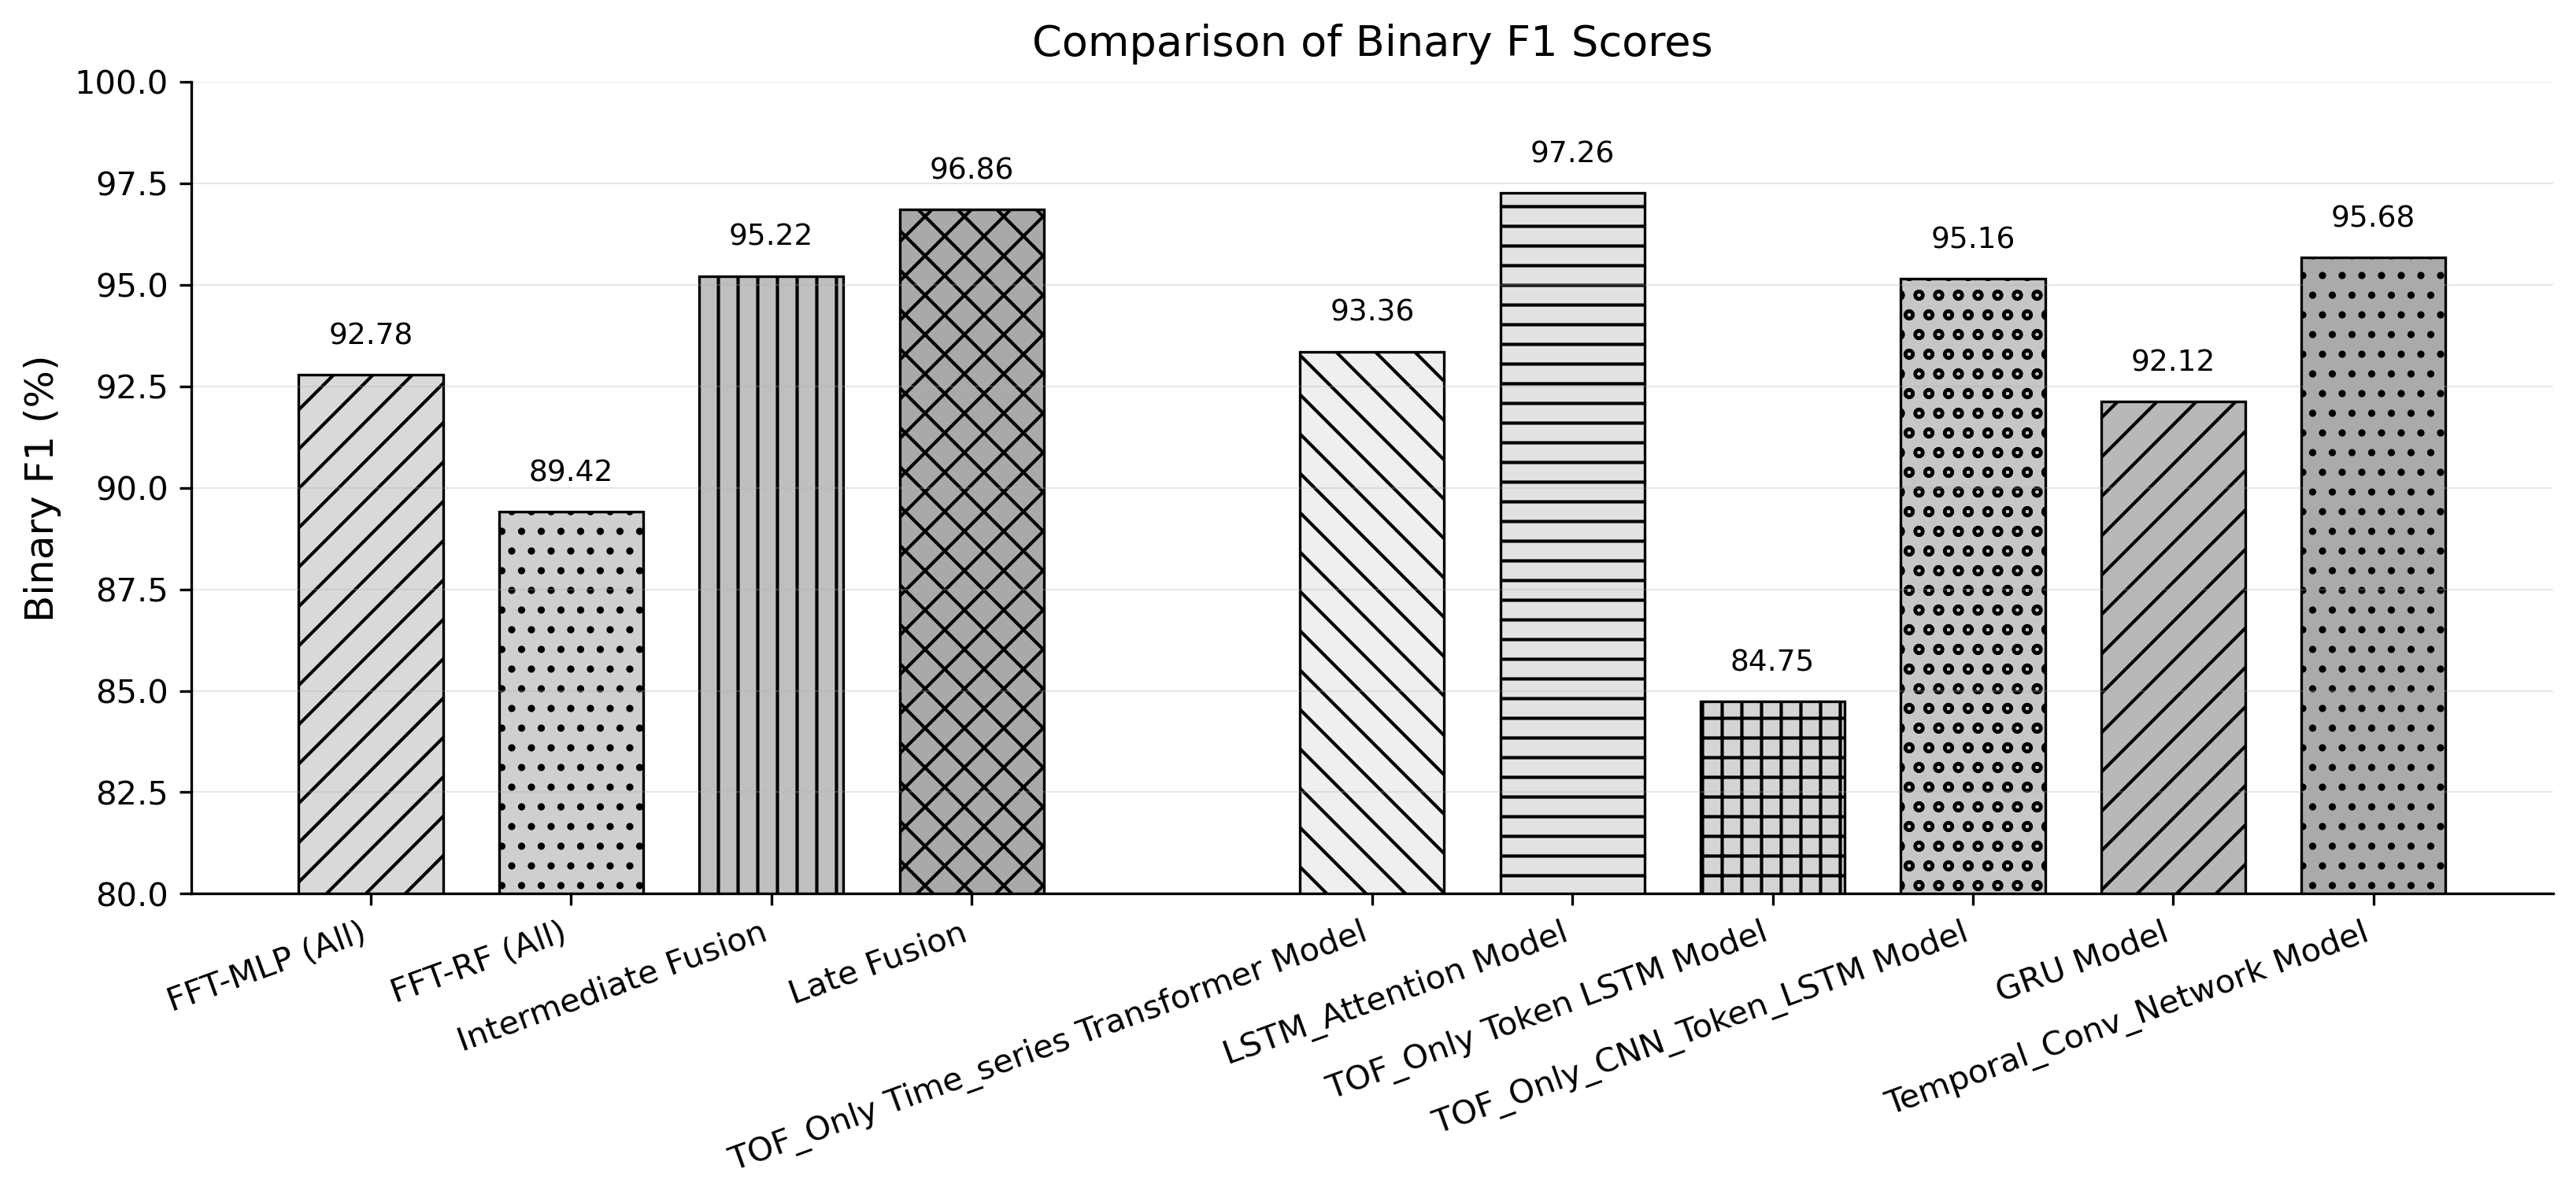
\includegraphics[width=\columnwidth]{model7_to_12_vs_baselines_binary_f1.png}
    \caption{Binary F1-score comparison between proposed NLP-based models and reproduced baselines. \cite{Hunter:2007}}
    \label{fig:Overall_binary}
\end{figure}

Figure~\ref{fig:Overall_binary} compares the binary F1-scores of the baseline models and the newly implemented models. Among the baseline methods, the late fusion model achieves the highest binary F1-score at 96.86\%, followed by the intermediate fusion model at 95.22\%. This shows that combining complementary sensor representations is very effective for the binary task of distinguishing BFRB from non-BFRB gestures.

For the newly added models, the LSTM-Attention model gives the best binary F1-score at 97.26\%, which is slightly higher than the late fusion baseline. The Temporal Convolutional Network model and the TOF-Only CNN-Token-LSTM model also perform strongly, with scores of 95.68\% and 95.16\%, respectively. In comparison, the TOF-only time series transformer reaches 93.36\%, which is higher than the FFT-RF baseline and close to the FFT-MLP baseline, but still below the strongest fusion-based and attention-based models.

One clear pattern in Figure~\ref{fig:Overall_binary} is that binary F1-scores are generally high across several models. This suggests that separating BFRB gestures from non-BFRB gestures is a relatively easier problem than fine-grained gesture classification. In the binary setting, many gesture differences inside each group are ignored, so the model mainly needs to learn a coarser boundary between harmful repetitive behaviors and ordinary actions. This is likely why several models can achieve binary F1-scores above 95\%.

For the TOF-only transformer, the result indicates that TOF signals alone carry useful information for BFRB detection, but they may not be sufficient to match the best multimodal or enhanced sequence models. A possible reason is that the transformer only uses TOF-based proximity patterns, while the stronger models either combine multiple modalities or use sequence structures that are better tuned to the dataset. Even so, the transformer result still shows that a TOF-only sequence model can provide competitive binary detection performance without relying on IMU or thermopile inputs.

\subsection{Macro F1-Score Comparison}



Figure~\ref{fig:Overall_macro} shows the macro F1-scores of all compared models. In contrast to the binary results, the macro F1-scores are much lower overall, which means that distinguishing among multiple gesture classes is more difficult than simply separating BFRB from non-BFRB behavior.

\begin{figure}[!htbp]
    \centering
    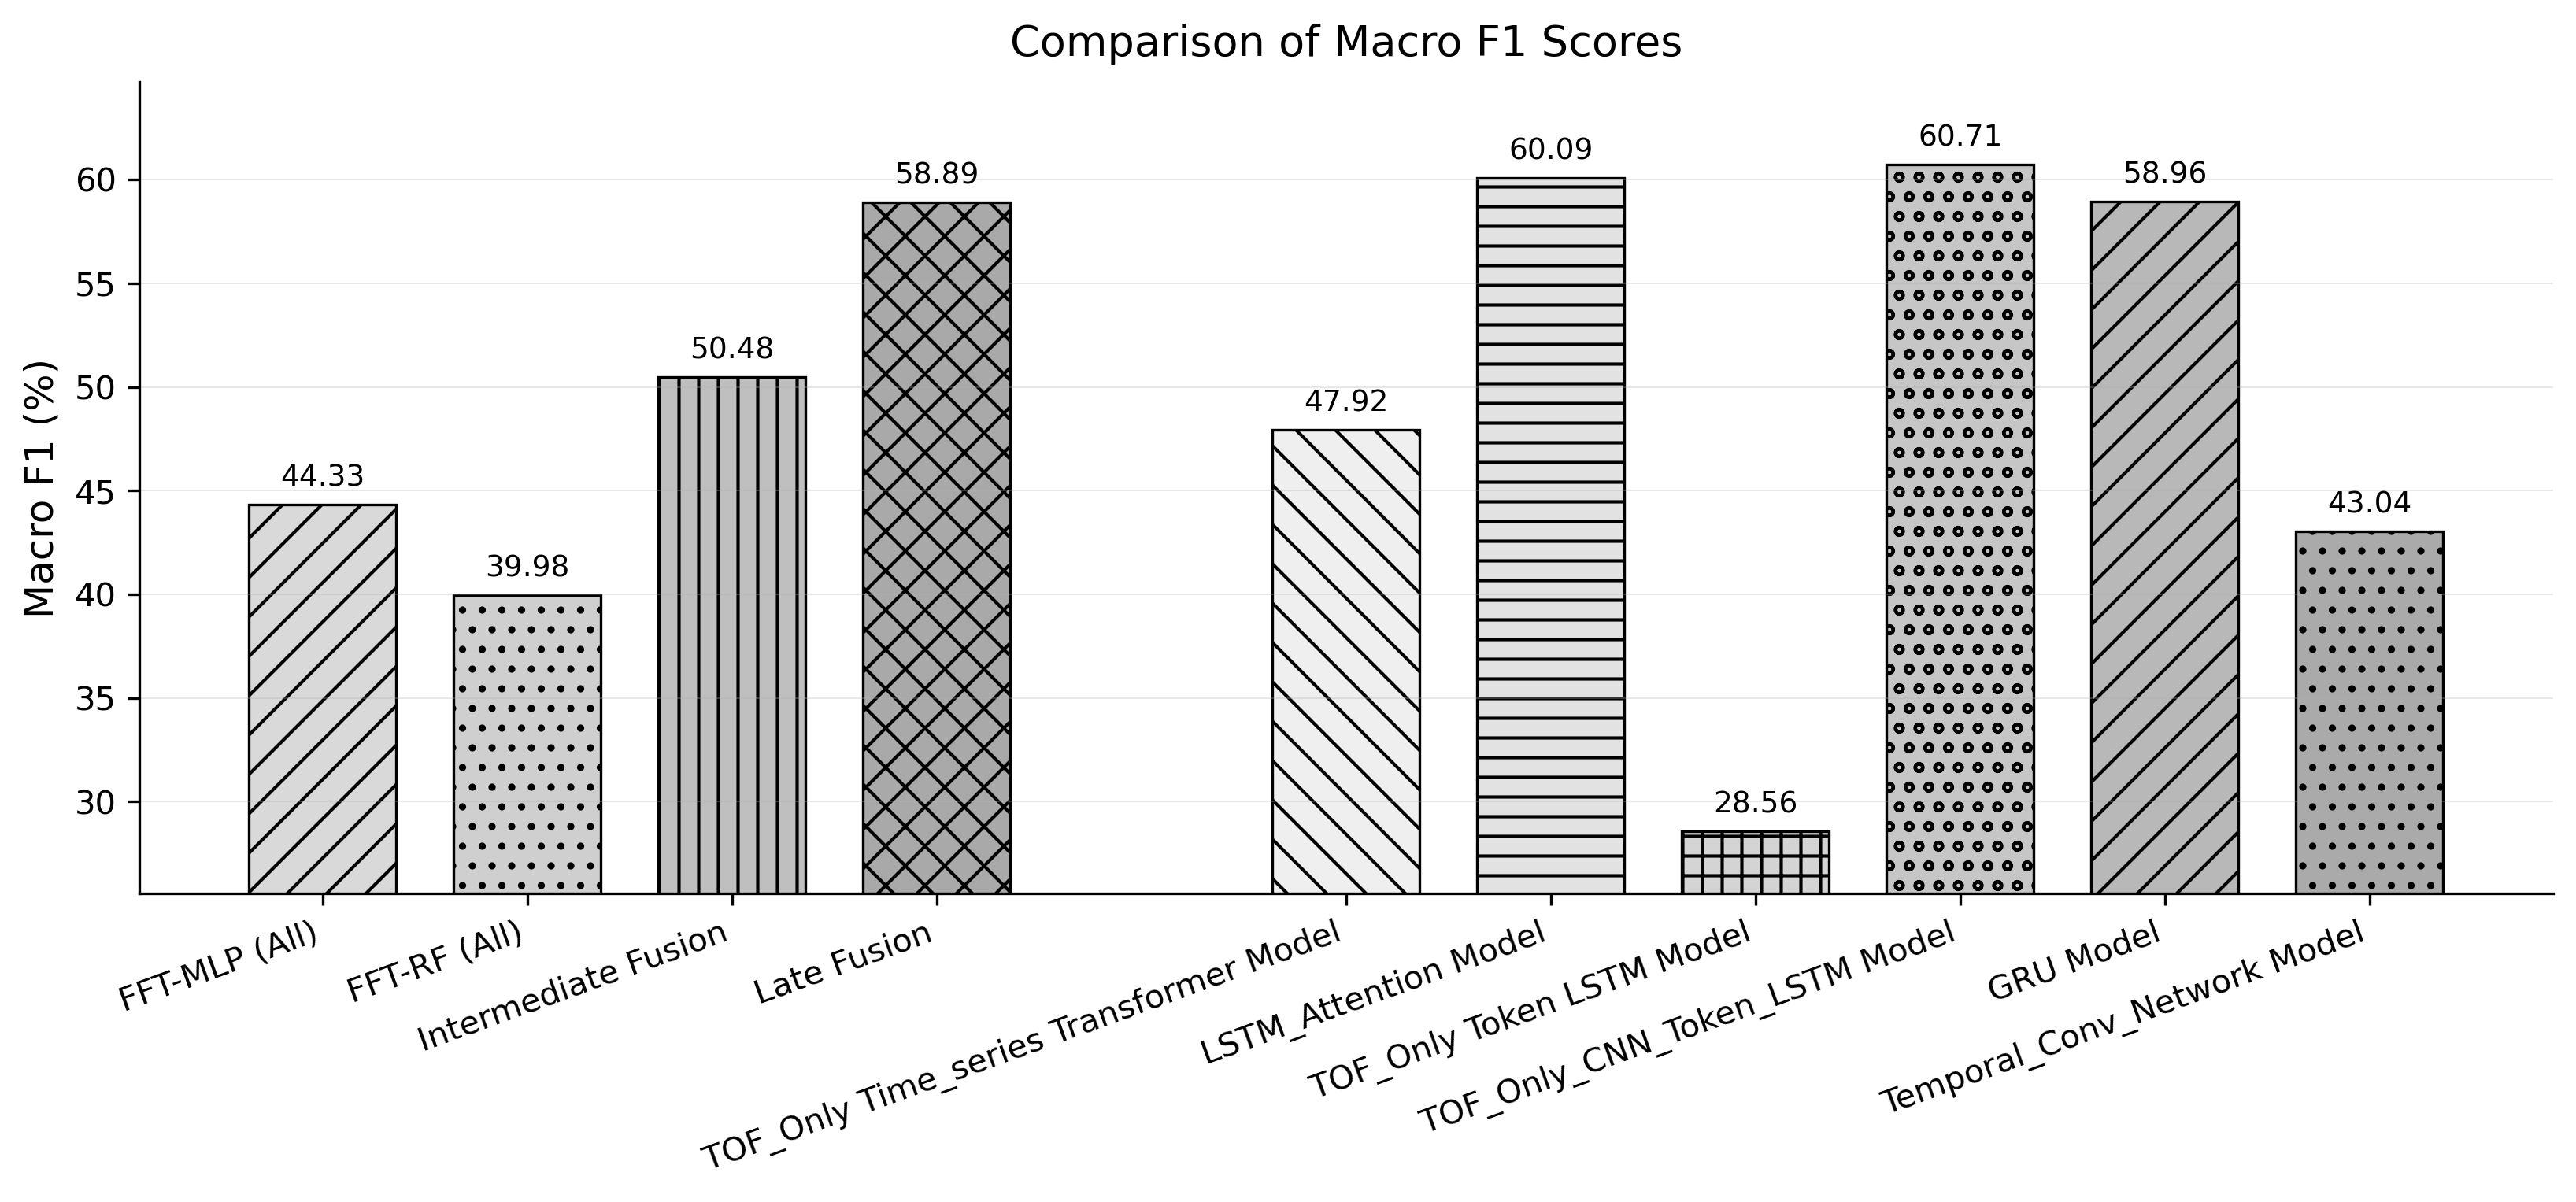
\includegraphics[width=\linewidth,height=2.5in,keepaspectratio]{model7_to_12_vs_baselines_macro_f1.png}
    \caption{Macro-averaged F1-score comparison between proposed NLP-based models and reproduced baselines \cite{Hunter:2007}.}
    \label{fig:Overall_macro}
\end{figure}


Among the baseline models, the late fusion model again performs the best, with a macro F1-score of 58.89\%, followed by the intermediate fusion model at 50.48\%. The FFT-based baselines are clearly lower, especially the FFT-RF model at 39.98\%. These results suggest that the fusion-based architectures are better able to preserve class-discriminative information than models that rely only on global FFT features.

For the new models, the TOF-Only CNN-Token-LSTM model achieves the highest macro F1-score at 60.71\%, slightly above the LSTM-Attention model at 60.09\% and the GRU model at 58.96\%. The TOF-only time series transformer reaches 47.92\%, which is again better than the FFT-RF baseline and slightly above the FFT-MLP baseline, but still below the strongest sequence models. The Temporal Convolutional Network model drops to 43.04\%, and the TOF-Only Token LSTM model performs the worst at 28.56\%.

Compared with the binary F1 results, the drop in macro F1 is expected. Many gestures in this dataset are similar in hand position, contact region, or movement pattern, so models can confuse one BFRB class with another even if they can still correctly identify that the gesture belongs to the BFRB group. Macro F1 is more sensitive to this type of confusion because it gives equal importance to each class instead of rewarding only the overall positive-versus-negative separation.

For the TOF-only transformer, the macro F1 result suggests that the model can learn some useful temporal structure from the TOF sequence, but fine-grained gesture recognition remains challenging when only TOF data are used. Since TOF mainly reflects proximity-related information, it may miss motion details that are useful for separating similar gestures. This may explain why the transformer is more competitive on binary F1 than on macro F1.



\subsection{TOF-Only Transformer versus the TOF Baseline}

Figure~\ref{fig:tof_only_binary_f1} compares the binary F1-scores of the TOF-only transformer and the TOF-only CNN-BiLSTM baseline reported in the paper. The transformer achieves 93.71\%, which is slightly lower than the 94.05\% of the CNN-BiLSTM model. Although the gap is small, this result suggests that the transformer did not fully outperform the baseline in the TOF-only setting.

\begin{figure}[!htbp]
    \centering
    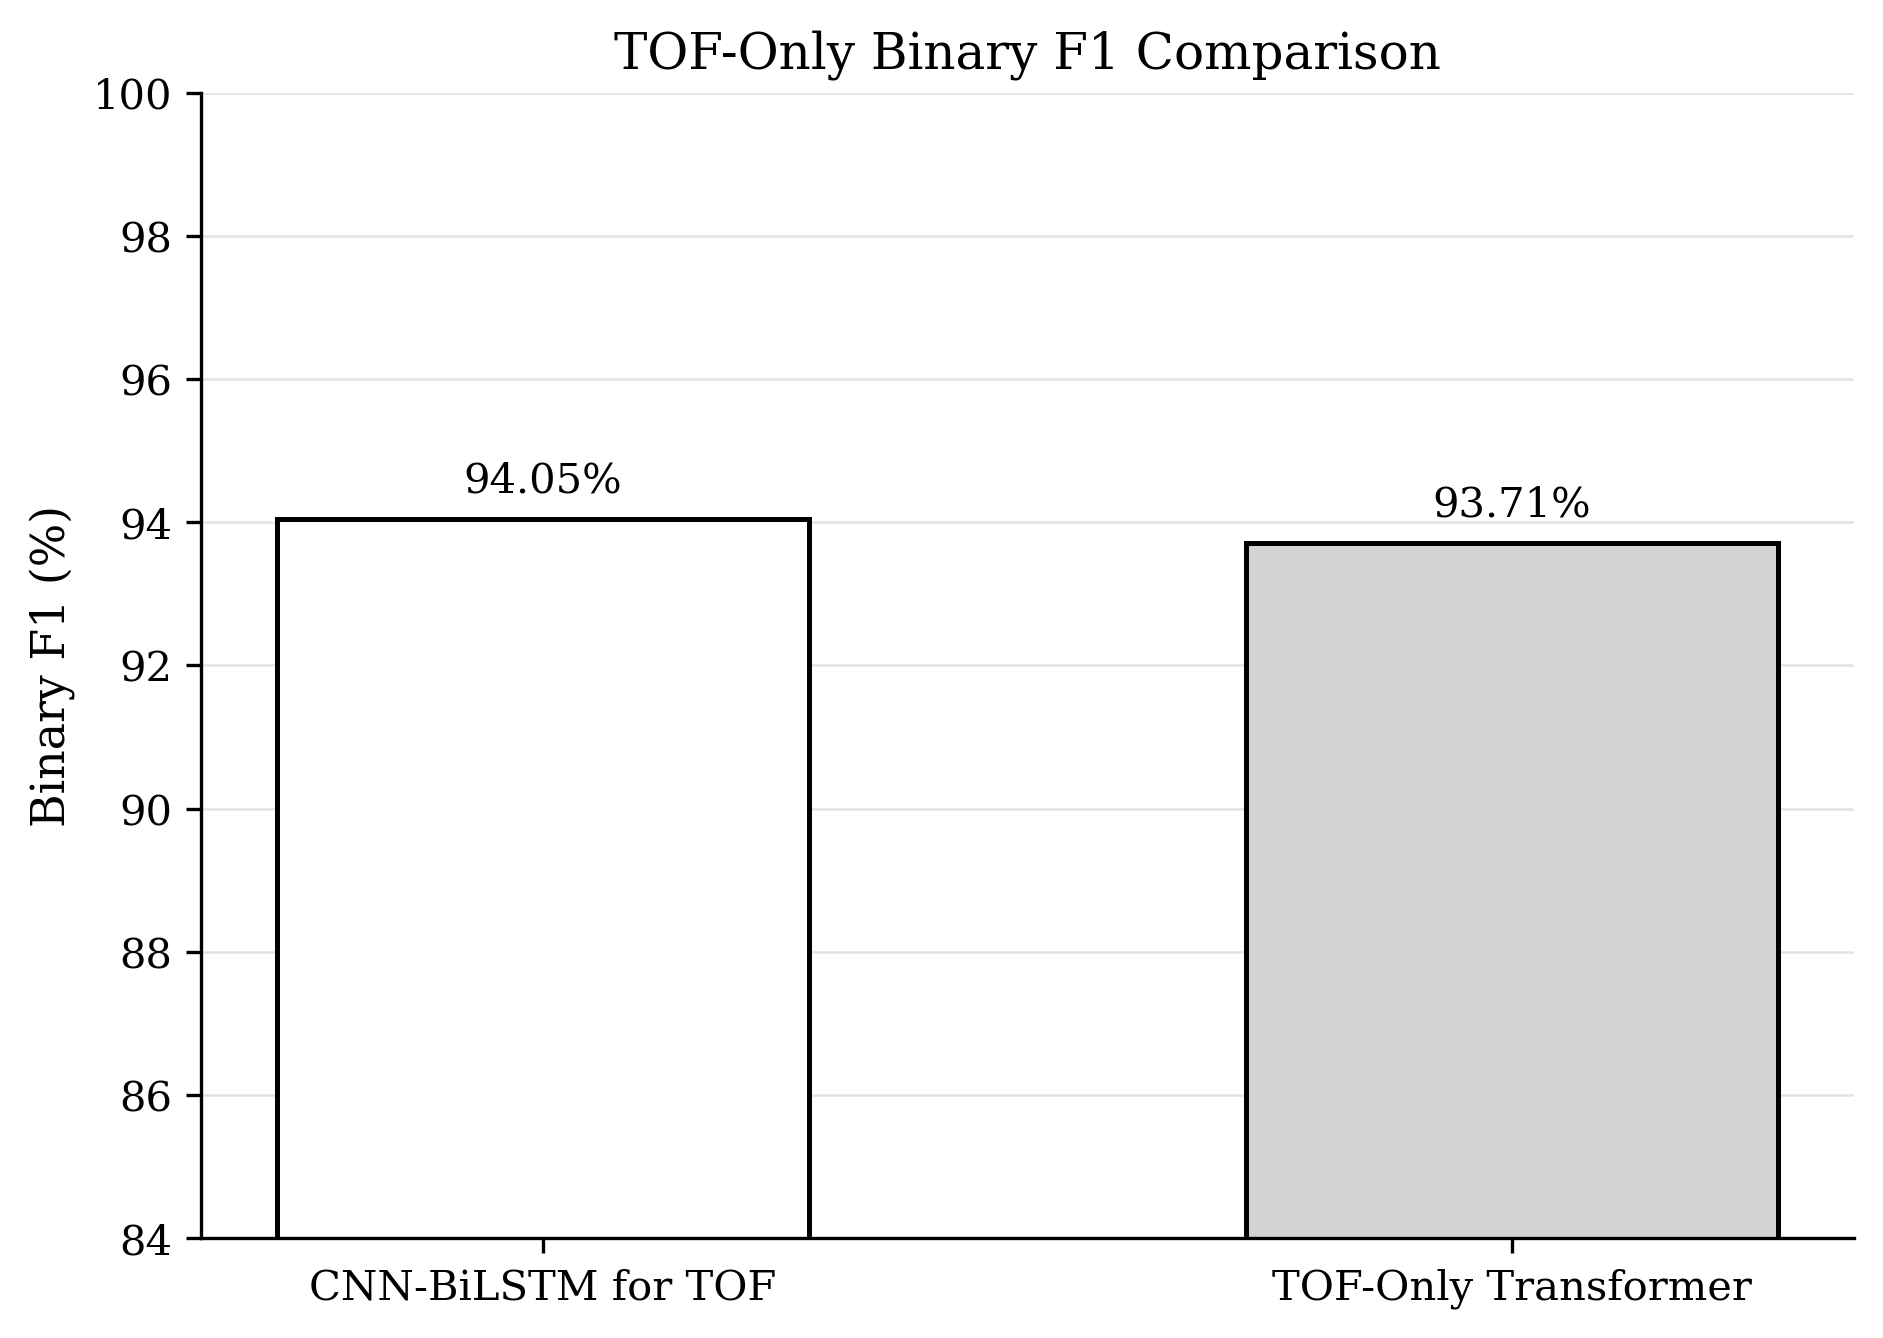
\includegraphics[width=\linewidth]{tof_only_binary_f1.png}
    \caption{TOF-Only Binary F1 Comparison.}
    \label{fig:tof_only_binary_f1}
\end{figure}

One possible reason is that the CNN-BiLSTM architecture is more closely matched to the structure of the TOF input. In the baseline model, each TOF reading is reshaped into spatial grids and processed by convolutional layers before temporal modeling with BiLSTM \cite{zhang2025bfrb}. This design preserves local spatial structure and then captures temporal dependencies across the gesture sequence. In contrast, our transformer follows the standard self-attention framework \cite{vaswani2017attention} and treats each time step mainly as a token in a sequence. This is effective for modeling global temporal relationships, but it does not explicitly exploit the local spatial arrangement inside each TOF reading as strongly as the CNN-based pipeline.

Another likely reason is that transformer models usually show their strengths when large amounts of training data are available. Prior work on time-series transformers has shown that self-attention is powerful for multivariate sequence modeling, but its performance is often influenced by sequence representation and data scale \cite{zerveas2021transformer}. In our case, the TOF-only dataset is more limited than the large-scale settings where transformers are often most competitive. Under this condition, the CNN-BiLSTM baseline may learn useful local and temporal patterns more efficiently.

In addition, our transformer uses fixed-length sequence construction with padding and masking, while the original gesture sequences have variable lengths. Although masking prevents padded positions from directly affecting attention, truncation and padding may still remove or weaken useful temporal details for some gestures. This can be especially important in TOF-only classification, where subtle changes in proximity over time may be critical for distinguishing BFRB from non-BFRB behaviors.



Overall, the result shows that the TOF-only transformer is still competitive, since its binary F1-score remains close to the published baseline. However, the CNN-BiLSTM architecture appears to be slightly better suited to this specific TOF-only task because it combines spatial feature extraction and temporal modeling in a way that aligns more naturally with the structure of the Helios TOF data \cite{zhang2025bfrb}.



\FloatBarrier
\subsection{Analysis of Temporal Convolutional Network}

To further understand the behavior of convolution-based sequence modeling, we analyze the performance of the Temporal Convolutional Network. The model achieves a Binary F1-score of 95.68\% and a Macro F1-score of 43.04\%.

\begin{figure}[!htbp]
    \centering
    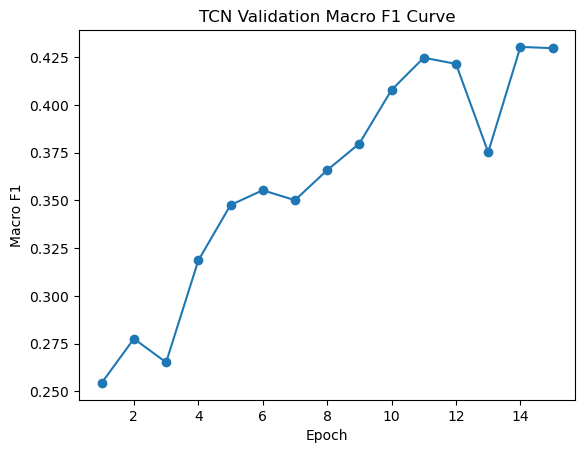
\includegraphics[width=\linewidth]{model10_tcn_macro_f1.png}
    \caption{Validation Macro F1-score over training epochs for the TCN model.}
    \label{fig:tcn_macro_f1}
\end{figure}

As shown in Figure~\ref{fig:tcn_macro_f1}, the validation Macro F1-score increases steadily from approximately 0.25 to 0.43 over the training process, reaching its peak at epoch 14. This indicates that the model is able to learn useful temporal patterns and converges in a stable manner without severe overfitting. However, the improvement slows down in later epochs, suggesting that the model approaches its performance limit.



The confusion matrix in Figure~\ref{fig:tcn_confusion} provides further insight into the model’s limitations. While several classes are predicted with high accuracy, there is noticeable confusion among gesture classes that share similar temporal patterns or spatial characteristics. This supports the observation that TCN is effective at capturing general temporal structure but struggles to distinguish fine-grained differences between similar gestures.

\begin{figure}[!htbp]
    \centering
    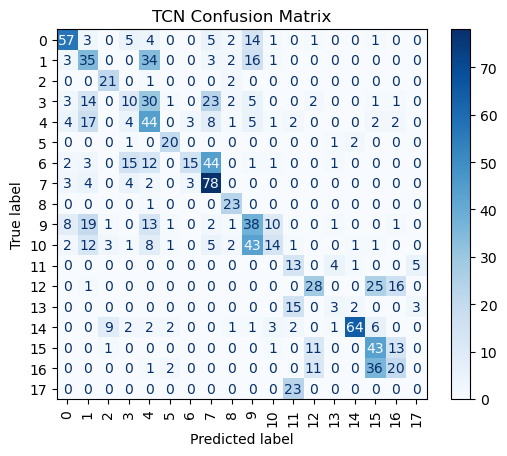
\includegraphics[width=\linewidth]{model10_tcn_confusion_matrix.png}
    \caption{Confusion matrix of the TCN model on the validation set.}
    \label{fig:tcn_confusion}
\end{figure}

The results indicate that TCN is a strong and efficient model for binary classification, but its performance in multi-class settings is limited compared to attention-based and hybrid sequence models. This aligns with the trends observed across all models, where fine-grained gesture recognition remains a more challenging task.

Compared to the TOF-only CNN-BiLSTM baseline reported in Zhang et al. \cite{zhang2025bfrb}, which explicitly models spatial structure within each TOF frame before temporal modeling, the TCN operates directly on flattened temporal sequences. While this allows efficient temporal pattern learning, it may limit the model’s ability to capture fine-grained spatial variations, which could contribute to the lower macro F1 performance observed in multi-class classification.

\FloatBarrier
\subsection{Analysis of GRU Model}

To further evaluate recurrent-based sequence modeling, we analyze the performance of the GRU model. The GRU achieves a Binary F1-score of 95.10\% and a Macro F1-score of 58.96\%, which is comparable to the LSTM-Attention model and slightly lower than the best-performing CNN-Token-LSTM model.

\begin{figure}[!htbp]
    \centering
    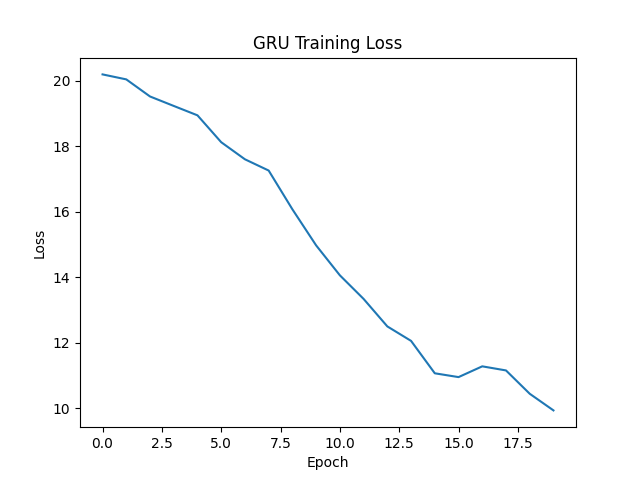
\includegraphics[width=\linewidth]{model7_gru_macro_f1.png}
    \caption{Training loss over epochs for the GRU model.}
    \label{fig:gru_macro_f1}
\end{figure}

As shown in Figure~\ref{fig:gru_macro_f1}, the GRU model demonstrates a stable training process, with the training loss decreases steadily over epochs and converges after several iterations. This indicates that the model is able to effectively learn temporal dependencies from the sequential sensor data without severe overfitting.

Compared to LSTM-based models, GRU uses a simplified gating mechanism with fewer parameters, which allows faster training and reduced computational complexity. Despite this simplification, the GRU achieves competitive performance, suggesting that complex gating structures may not be strictly necessary for capturing temporal patterns in this dataset.

However, similar to other sequence models, the GRU shows limitations in multi-class classification. The relatively lower Macro F1-score suggests that the model struggles to distinguish between gesture classes with similar temporal dynamics. Since GRU primarily focuses on temporal dependencies, it may not fully capture fine-grained spatial variations present in TOF sensor data.

Compared to the CNN-BiLSTM baseline reported in Zhang et al. \cite{zhang2025bfrb}, which explicitly models spatial structure using convolutional layers before temporal modeling, the GRU operates directly on flattened sequences. This design simplifies the architecture but may limit its ability to extract spatially structured features, which could explain the gap in fine-grained classification performance.

\begin{figure}[!htbp]
    \centering
    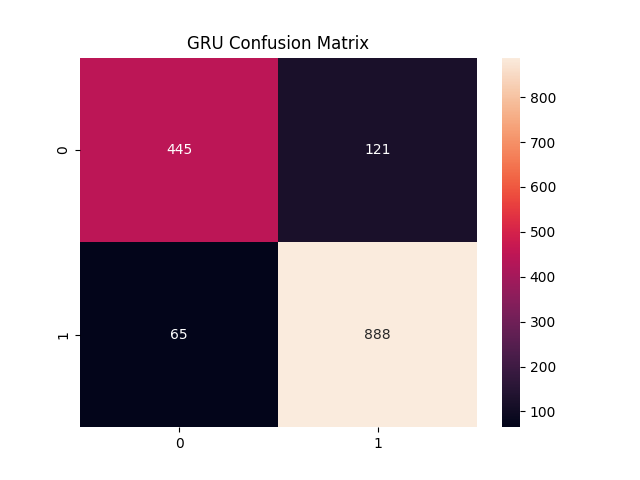
\includegraphics[width=\linewidth]{gru_confusion_matrix.png}
    \caption{Confusion matrix of the GRU model on the validation set.}
    \label{fig:gru_confusion}
\end{figure}

The confusion matrix further shows that misclassification mainly occurs among similar BFRB classes, reinforcing the difficulty of fine-grained gesture recognition.

\clearpage
\section{Discussion}

Our experimental results show that NLP-inspired sequence modeling methods provide a meaningful extension to prior work on Body-Focused Repetitive Behavior (BFRB) detection from wearable sensor data. The proposed models confirm that temporal sequence learning is effective for distinguishing BFRB from non-BFRB behaviors, while fine-grained gesture classification remains substantially more difficult. This difference is important because a practically useful system should not only detect problematic behavior in general, but also distinguish among different BFRB types with sufficient reliability. Overall, the results suggest that sequence-based architectures are well aligned with the temporal structure of Helios sensor streams, but model improvements alone are not enough to overcome limitations caused by class overlap, data structure, and sensor-specific constraints.

One of the clearest findings is the persistent gap between binary F1-score and macro-averaged F1-score across both reproduced baselines and newly proposed models. In the binary setting, the task is coarse-grained, requiring only a distinction between BFRB and non-BFRB gestures. Under this formulation, many within-class differences are ignored, allowing strong temporal models to achieve high scores. In contrast, macro F1 requires the model to separate multiple gesture classes that often share similar motion trajectories, contact regions, and temporal patterns. For example, scratching, pulling, or pinching near nearby facial or neck regions may produce highly similar sensor signals. This explains why several models perform strongly in binary classification but show only limited gains in multi-class classification.

The differences among architectures also provide insight into how model design interacts with multimodal wearable data. Recurrent models such as GRU and LSTM are naturally suited to sequential sensor inputs because they aggregate information over time and preserve temporal context. In our experiments, these models perform well when the task is to capture broad temporal patterns associated with repetitive behavior. Attention-enhanced models further improve this idea by allowing the network to emphasize more informative time steps rather than treating all positions equally. This is useful in BFRB detection because short moments of contact, transition, or localized motion may carry more discriminative information than the rest of a sequence. Hybrid architectures such as CNN-Token-LSTM are especially promising because they combine local pattern extraction with temporal modeling, capturing both short-range motifs and longer dependencies.

By contrast, the transformer-based model shows more mixed results. In principle, self-attention is attractive for multivariate time series because it allows each time step to interact directly with all others. However, our experiments suggest that this flexibility does not automatically produce better performance in this task. A likely reason is that transformer models often require larger datasets, longer effective sequences, or stronger input representations to clearly outperform simpler sequence models. In our case, the fixed-length representation, padding, and TOF-only constraint may have limited the transformer's advantage. This does not mean transformers are unsuitable for BFRB detection, but rather that they may require stronger multimodal fusion, pretraining, or better structural inductive biases in this domain.

Compared with the baseline study of Zhang et al.~\cite{zhang2025bfrb}, our findings both reinforce and extend the earlier conclusions. The strong performance of fusion-based baselines remains convincing evidence that combining complementary sensor modalities is effective for BFRB detection. At the same time, our results show that NLP-inspired sequence models can match or slightly exceed baseline performance without relying only on the original frequency-domain pipeline. This suggests that the problem can benefit not only from classical signal processing, but also from modern sequence modeling perspectives. However, because macro F1 remains difficult even for stronger models, the main bottleneck may now lie less in model family and more in whether the representation can adequately separate highly similar gesture categories.

Several limitations should be acknowledged. First, the study relies on a single dataset, so the conclusions may not fully generalize to other devices, populations, or real-world environments. Second, fixed-length padding and truncation may remove useful temporal information, especially when discriminative patterns occur near sequence boundaries or vary in duration. Third, class imbalance remains a challenge because rare gesture categories provide fewer examples for stable learning. Fourth, evaluation is performed offline rather than in a real-time deployment setting, so latency, efficiency, and robustness to noise remain open questions. Fifth, there are trade-offs between performance and deployability, since more expressive sequence models may also increase inference cost, memory usage, and tuning complexity. It shows that BFRB detection is a useful testbed for studying how NLP-inspired sequence models transfer to multimodal health-related time series. The results suggest that no single architecture is universally dominant; performance depends on how well model inductive biases align with the temporal and structural properties of the sensor data. This insight may also be relevant to activity recognition, digital phenotyping, assistive monitoring, and other healthcare sensing tasks requiring fine-grained temporal discrimination.

If this work continues over the next six months, several directions would be especially worthwhile. On the data side, collecting more diverse recordings, improving class balance, and designing augmentation methods for wearable sequences would likely strengthen generalization. On the modeling side, more advanced multimodal fusion methods, lightweight attention mechanisms, and stronger representation-learning strategies could improve the balance between accuracy and efficiency. On the evaluation side, cross-subject validation, calibration analysis, threshold tuning, and real-time deployment experiments should be prioritized to better reflect practical use. Together, these directions would move the project from a strong experimental comparison toward a more robust and deployable BFRB detection system.

\clearpage
\section{Conclusion}

In conclusion, this work reproduced the main BFRB detection baselines and extended them with NLP-inspired sequence models under a unified evaluation pipeline. The experimental results show that sequence-based architectures are highly effective for modeling temporal patterns in wearable sensor data, achieving consistently strong performance in binary classification tasks across multiple model designs. In particular, attention-enhanced and hybrid models demonstrate competitive results, highlighting the importance of capturing both long-range temporal dependencies and local signal structures. However, the results also reveal a clear limitation: while binary F1-scores are high, macro-averaged F1-scores remain significantly lower, indicating that fine-grained gesture classification across multiple BFRB categories is still challenging. This suggests that model improvements alone are not sufficient to fully address the complexity of the task, and that issues such as class similarity, data imbalance, and limited representation diversity play a critical role in performance. Our findings suggest that combining modern sequence modeling techniques with improved data representation and multimodal fusion strategies is a promising direction for advancing BFRB detection. Furthermore, the unified experimental framework developed in this work provides a reproducible basis for systematically comparing different model families under consistent conditions. Overall, this study demonstrates the applicability of NLP-inspired models to time-series sensor data and provides practical insights into their strengths and limitations, offering a foundation for future research in multimodal and sequence-modeling approaches for wearable BFRB detection.



\clearpage
\appendices 
\section{} \begin{figure}[!htbp] \centering 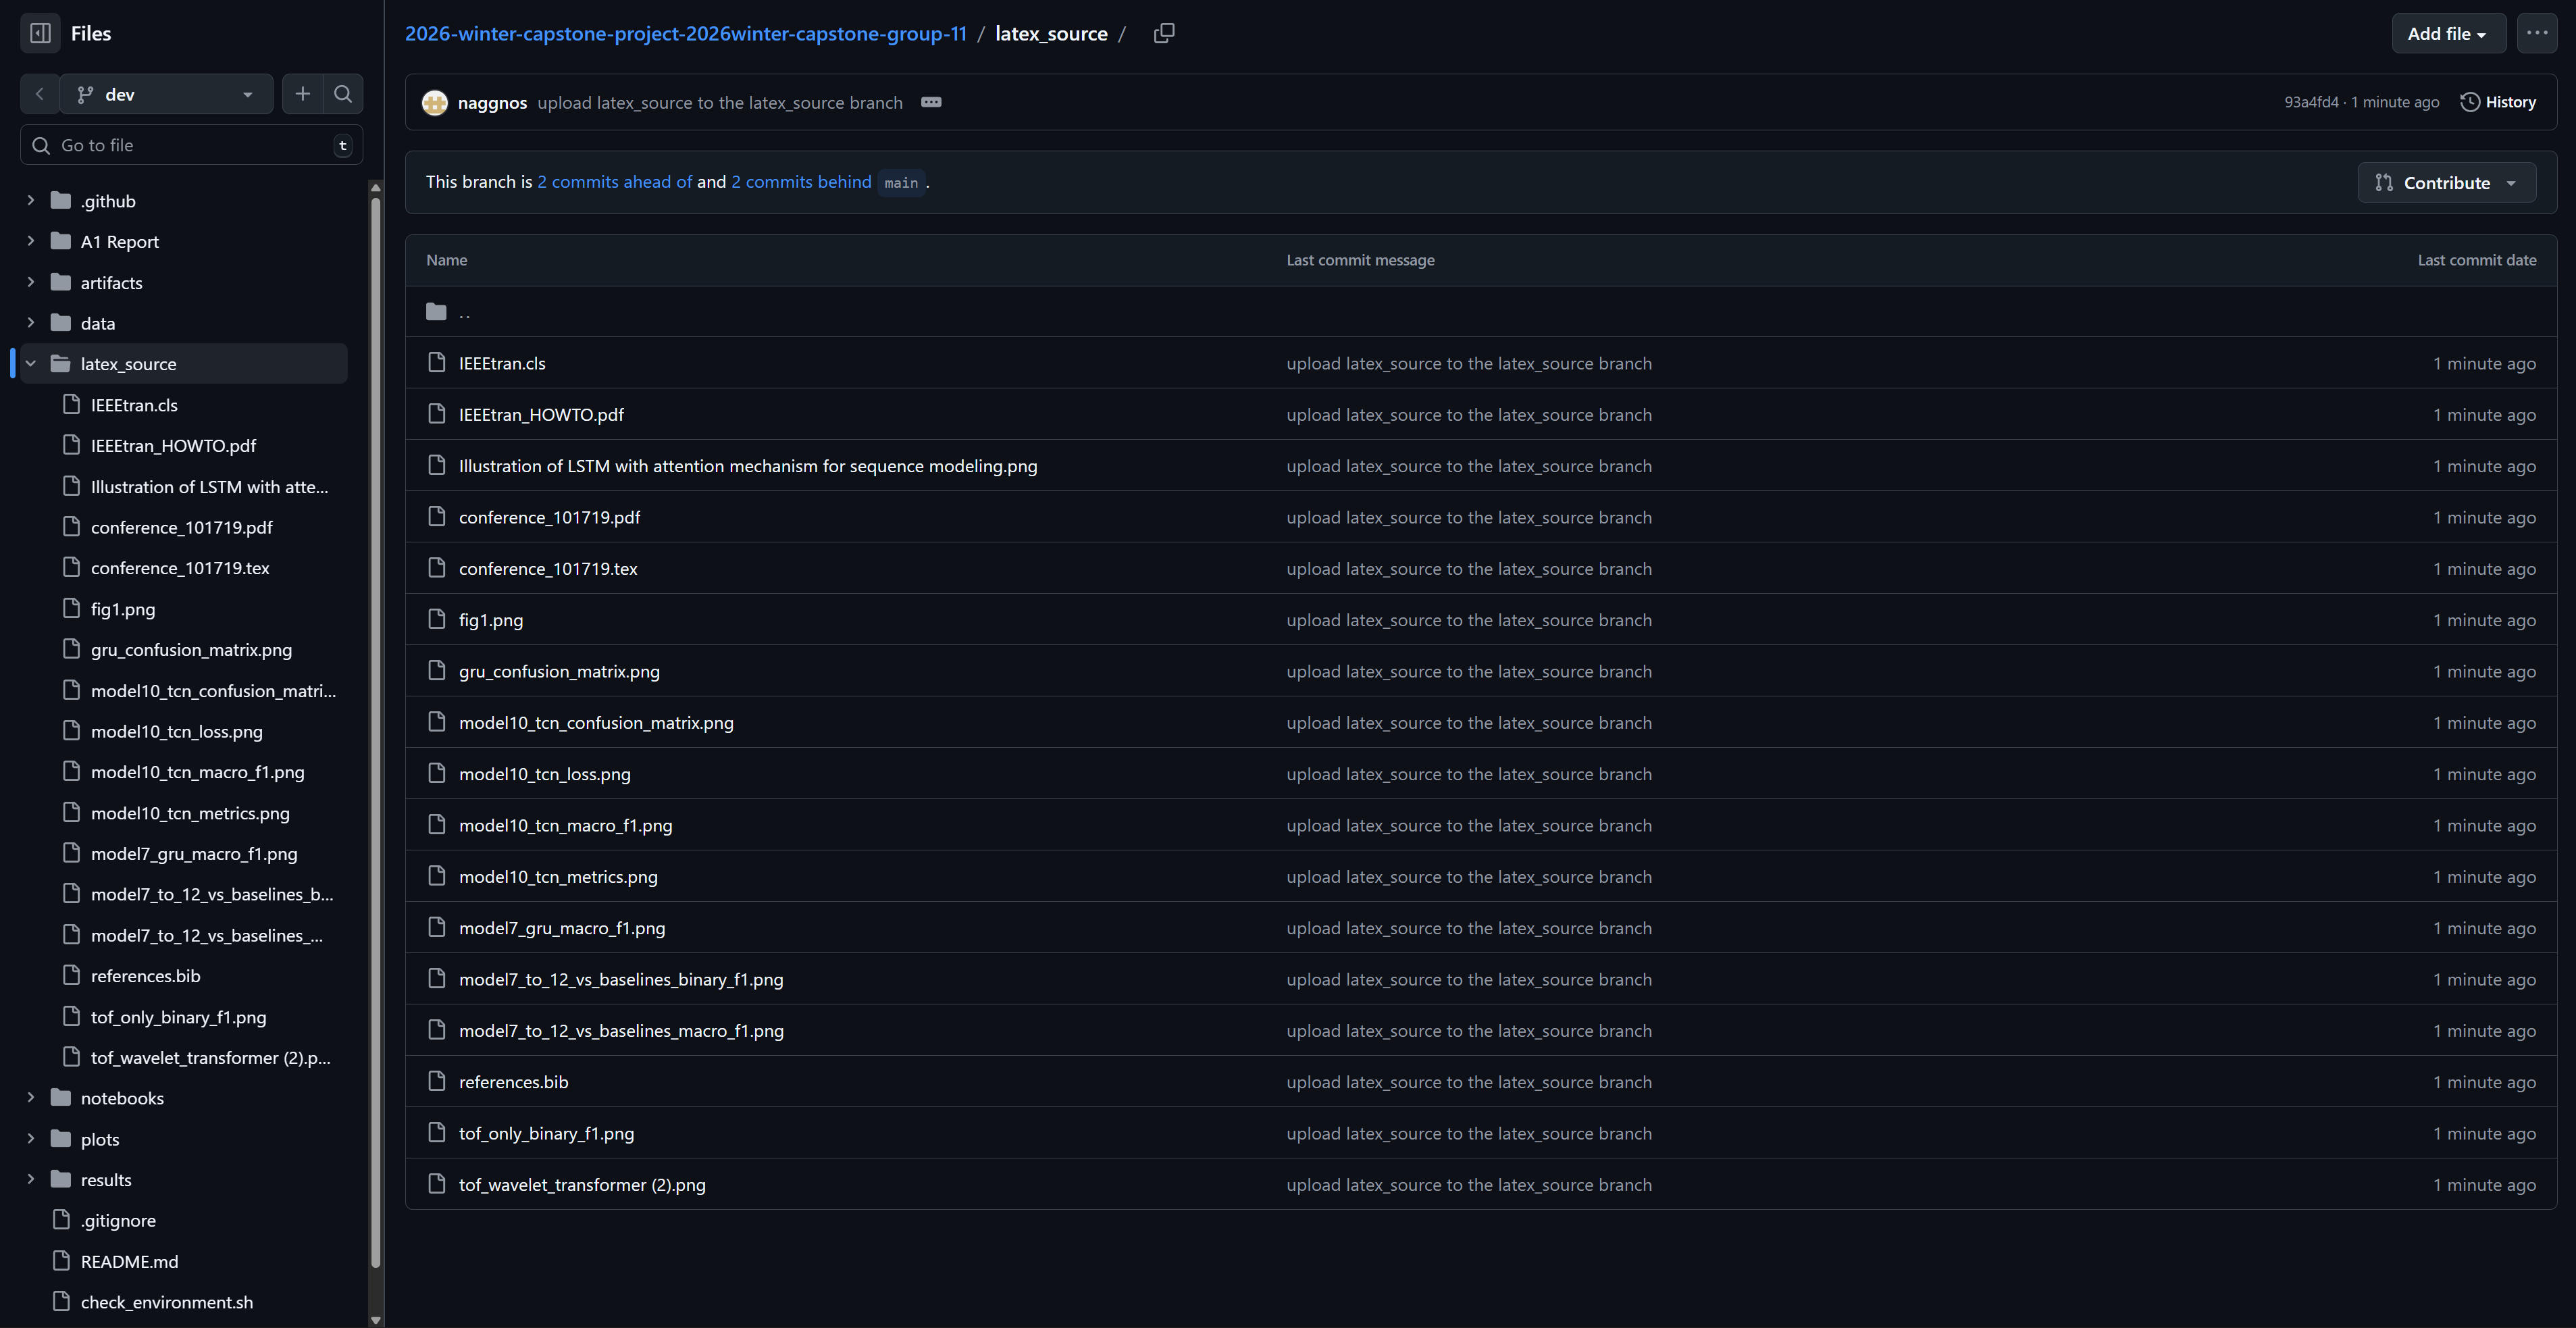
\includegraphics[width=\linewidth]{Screenshot 2026-04-14 091103.png} \caption{Screenshot for the latex-source.} \end{figure}

\clearpage
\bibliographystyle{IEEEtran}
\bibliography{references}

\end{document}